%%%%%%%%%%%%%%%%%%%%%%%%%%%%%%%%%%%%%%%%%%%%%%%%%%%%%%%%%%%%%%%%%%%%%%%%%%%%%%%
% CAPÍTULO 3 - GESTIÓN DE CÓDIGO Y PROCESO DE DESARROLLO
%%%%%%%%%%%%%%%%%%%%%%%%%%%%%%%%%%%%%%%%%%%%%%%%%%%%%%%%%%%%%%%%%%%%%%%%%%%%%%%
\chapter{Gestión de código y proceso de desarrollo}
\label{chap:codeManagement}
\begin{comment}
Introducción de lo que es el proyecto, lo del libro de Python y luego las tecnologías usadas en el proyecto unidas con la introducción.
\end{comment}
En este capítulo trataremos como está compuesto el proyecto y como se ha gestionado este, tanto la parte del código fuente de nuestro paquete \emph{PyCardio} como el código que forma parte de nuestro proyecto web reflejando todo lo que concierne a \emph{PyCardio} como documentación, como usarlo, funcionalidades. \\
Para ello dividiremos el capítulo en tres secciones:
\begin{enumerate}
    \item Explicación de que contiene el proyecto \emph{PyCardio} mediante un resumen y un esbozo de lo que mostraremos en la página web.
    \item Buenas prácticas de desarrollo en Python y como escribir buen código.
    \item Identificación de los elementos de nuestro proyecto con las tecnologías descritas en el capítulo \ref{chap:Arqui}, para la gestión de proyecto del Backend.
\end{enumerate}

        %%%%%%%%%%%%%%%%%%%%%%%%%%%%%%%%%
        %% EXPLICACIÓN DE CONTENIDO
        %%%%%%%%%%%%%%%%%%%%%%%%%%%%%%%%%
\subsection{¿Que és PyCardio?}
\label{subsec:explainPyCardio}
\emph{PyCardio} es un módulo en desarrollo  de Python creado por el Dr. Óscar Barquero. Dicho módulo tiene el objetivo de realizar análisis de las señales cardíacas, es decir:
\begin{itemize}
    \item \textbf{ECG Análisis}: Detección del complejo QRS, extracción de series temporales de intervalo RR, delinación completa de ECG.
    \item \textbf{Análisis de variabilidad de la frecuencia cardíaca}: Un análisis completo de las series temporales de intervalo RR, donde se realiza un preprocesado, análisis en  el dominio del tiempo, análisis en el dominio de la frecuencia, análisis no lineal y un análisis tiempo-frecuencia.
    \item \textbf{Análisis de la frecuencia cardiaca de turbulencia.}
    \item \textbf{Análisis de fibrilación auricular.}
    \item \textbf{Análisis de fibrilación ventricular.}
    \item \textbf{Análisis de arritmia mediante 24 Holter.}
\end{itemize}

El objetivo, por tanto, es la creación de una página web que muestre estas funcionalidades, así como una guía de instalación, documentación, y una orientación de como colaborar en el proyecto mediante las tecnologías mencionadas en el capítulo \ref{chap:Arqui}.

[[ESBOZO DE LA WEB]]

    %%%%%%%%%%%%%%%%%%%%%%%%%%%%%%%%%%%%%%%
    %% BUENAS PRÁCTICAS DE DESARROLLO
    %%%%%%%%%%%%%%%%%%%%%%%%%%%%%%%%%%%%%%
\subsection{Buenas prácticas de desarrollo en Python}
\label{subsec:bestPracticses}
En esta sección tratamos de explicar y mostrar buenas prácticas para el desarrollo de proyectos en Python.\\

\subsection*{Estilo de código}
\label{subsec:stylePython}
Para los \emph{pythonistas} (desarrolladores veteranos de Python) el código fuente de un proyecto es mas leído que escrito, por tanto, el corazón de un proyecto Python es la le legibilidad. Una de las razones por las que el código Python es legible es por sus amplias guías de estilo (recogidas en PEP 8 y PEP 20). La comunidad Python intenta hacer lo posible para que sus proyectos se ajusten a estas guías. Tomando como ejemplo uno de los módulos que disponemos en \emph{PyCardio}, podemos ver cuanto sigue nuestro código las reglas de la guía PEP8. Para ello: 
\begin{lstlisting}[language=sh, caption=Ejemplo de PEP8 con \emph{PyCardio},label=pep8]
$ pep8 HRV.py
HRV.py:3:79: W291 trailing whitespace
HRV.py:5:80: E501 line too long (83 > 79 characters)
HRV.py:5:84: W291 trailing whitespace
HRV.py:6:80: E501 line too long (80 > 79 characters)
HRV.py:18:1: E302 expected 2 blank lines, found 1
HRV.py:19:1: W293 blank line contains whitespace
HRV.py:21:34: W291 trailing whitespace
HRV.py:23:1: W293 blank line contains whitespace
HRV.py:24:1: W293 blank line contains whitespace
HRV.py:25:5: E303 too many blank lines (2)
HRV.py:27:80: E501 line too long (89 > 79 characters)
\end{lstlisting}
Estas guías de código suelen integrarse en IDE para facilitarnos su seguimiento,o ejecutar el programa \texttt{autopep8}, que regenera el código siguiendo la guía PEP8.  

\subsection*{Estructurando el proyecto}
\label{subsec:structurePython}
Por una \emph{estructura} de proyecto de programación nos referimos a como la lógica y las dependencias del código están implementadas. \\
Por tanto seguir una buena estructura de empaquetado y de importar los módulos que se utilicen en el proyecto proporcionará un código menos repetitivo y desordenado. No hay una guía de como estructurar un proyecto pero los siguientes errores más comunes pueden ayudar a  como estructurarlo:
\begin{itemize}
    \item \textit{Dependencias circulares múltiples y desordenadas:} Ocurre cuando un módulo depende de otro, y este a su vez del mismo inicial. Es decir, \textit{fabrica.py} depende de \textit{trabajadores.py}, que depende de \textit{fabrica.py}.
    \item \textit{Un abuso en el uso de contextos globales:} Ocurre cuando para dos clases o módulos que hacen uso de la misma variables globales, haciendo así que cualquiera de los dos pueda modificarlo.
    \item \textit{Código Ravioli:} hace referencia a que el código se refactoriza en demasiados trozos.
\end{itemize}

Python a veces se describe como un lenguaje orientado a objetos, pero esto puede resultar engañoso ya que a diferencia de Java, no impone este paradigma de programación como principal. Por tanto, no es necesario definir clases para desarrollar un proyecto en Python, pero en algunas ocasiones es necesario mantener un estado o un contexto, es decir, necesitamos variables globales de clase. La recomendación a seguir es cuando nos querramos traer entre manos un código con contexto persistente o estado, debemos usar funciones o procedimientos con contextos implícitos y efectos secundarios \footnote{\textbf{Contexto implícito} refiere a código que necesita acceder a variables globales para su función, mientras que \textbf{efectos secundarios} es cuando una función o procedimiento cambia el valor  o estado de una variable global. } lo mínimo posible. Uno de los objetivos de desarrollar clases personalizadas es aislar funciones con contexto o efectos secundarios, para ello, se aconseja utilizar cuanto más sea posible la programación funcional, es decir, utilizar funciones puras \footnote{Las \textbf{funciones puras} son aquellas funciones que dada una entrada distinta producen la misma salida.}. Las ventajas de usar la programación funcional  a la hora de desarrollar un proyecto son:
\begin{itemize}
    \item Funciones puras son más sencillas de cambiar o reemplazar si se necesita una optimización.
    \item El uso de funciones puras facilita el desarrollo de tests sobre nuestro proyecto.
    \item El tener funciones puras hace más sencillo la manipulación y decoración de estas.
\end{itemize}
Como ya sabemos, Python es un lenguaje dinámicamente tipado, lo que quiere decir que una misma variable puede tomar un valor, e inmediatamente después puede ser una cadena de texto, o una función. Esta característica del lenguaje se considera una debilidad del lenguaje, ya que hace muy difícil trazar código.\\

\subsection*{Pruebas de código}
A la hora de distribuir software de código libre, una de las prácticas que hacen que el software sea más utilizado o que ayude a que se sumen contribuciones al software es la prueba del código. ¿Por qué es una de las prácticas para el desarrollo de un proyecto más importante?. Las siguientes razones son tanto para el ámbito comercial como para un ámbito práctico de desarrollo: 
\begin{itemize}
    \item Porque hasta que una línea de código no es ejecutada, no se puede saber si esta funciona.
    \item En la mayoría de los casos, el código no se ejecuta de principio a fin a menos que se pruebe con los distintos conjunto de casos que trata el software.
    \item Cuando el código es modificado por otros usuarios, es propenso a que este deje de funcionar de manera inesperada. La implementación de tests da la confianza de que a partir de estas modificaciones no se ha "roto" el software de manera inesperada.
    \item Porque ayuda a entender los cambios que se han realizado en el código.
    \item Las pruebas de código ayudan a optimizar tiempo y dinero, ya que uno de los beneficios que aporta el testeo de software es la rentabilidad. El desarrollo de software consiste en un trabajo por etapas, por tanto, cuanto antes se detecten los bugs más sencillo será tratarlos. 
    \item Uno de los puntos más importantes a la hora de confiar en un software es la seguridad, las pruebas de código ayudan al consumidor a ver que tienen delante un producto fiable, a que los problemas y riesgos del software son tratados de antemano, a obtener un producto libre de vulnerabilidades y a mantener datos personales de usuario seguros.
\end{itemize}

A raíz de todos los beneficios que trae el incorporar tests en el desarrollo de software, cada vez se adopta más en la ingeniería de software la práctica de programación TDD (Test-Driven Deployment). Esta consiste en escribir pruebas unitarias \footnote{Pruebas centradas en una única pieza de código como objeto, fúncion.} centrando estas pruebas en los requisitos para nuestro software, tras ello, se implementa el código adecuado para que dichas pruebas no fallen. El siguiente paso, una vez que nuestro código ha pasado las pruebas unitarias es refactorizarlo. Tras su refactorización se vuelve al punto de inicio abordando otro requisito de nuestro desarrollo. \\
\begin{figure}[h]
    \centering
    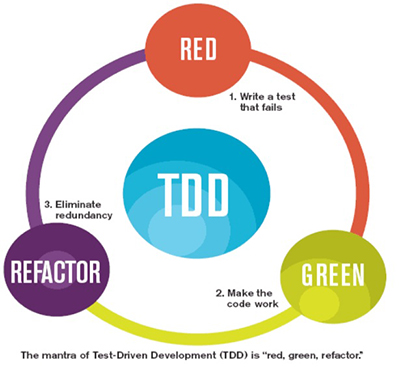
\includegraphics[scale=0.8]{img/TDD__logo.jpg}
    \caption{Esquema de práctica de programación de TDD (Test-Driven Deployment)}
    \label{fig:tdd}
\end{figure}
Seguir la práctica de programación TDD supone un cambio en la mentalidad de desarrollo, pensamos en qué queremos hacer con nuestro software y tras ello, cómo debe hacerlo. Adoptar esta metodología de trabajo es lenta, pero una vez adoptada el proceso de desarrollo es rápido y ágil. Afrontar el desarrollo mediante esta nueva práctica puede parecer un gasto de recursos debido al aprendizaje que supone adoptarla, pero esta es una inversión a largo plazo, ya que, ahorra recursos en el mantenimiento de nuestro código. Con TDD se garantiza una cobertura de código entre el 90\% y 100\%,lo que nos permite añadir funcionalidades de manera rápida y sencilla. Por último, esta forma de trabajo nos permite entender mejor el código y facilitar las contribuciones futuras en el software aumentando así la calidad del producto. 
\subsection*{Documentación}
Para un proyecto Python no solo se busca la legibilidad en el código, si no también en la documentación. A continuación se presentan unas buenas prácticas para facilitar tanto el uso como la contribución del proyecto. 
\subsubsection*{Documentación de  Proyecto}
Para cualquier proyecto de \emph{software} libre suele existir una documentación para usuarios y otra adicional para quien quiera contribuir al proyecto. Los siguientes ficheros que se comentan a continuación hacen referencia a esa documentación adicional y se centran en facilitar la contribución:\\
\begin{itemize}
    \item \textit{README}: Tal y como hemos mencionado, cuando creamos un repositorio GitHub es frecuente tener un fichero escrito en \emph{MarkDown} con el propósito de tener un breve resumen del contenido del proyecto o librería, la dirección del código principal. Este fichero es la entrada para cualquier usuario o contribuyente al proyecto. 
    \item \textit{INSTALL}: Este fichero es menos necesario en Python, ya que se reduce a ejecutar el comando \texttt{pip install [NAME\_MODULE]} o a ejecutar el script \emph{setup.py}. En él se añaden las instrucciones de instalación.
    \item \textit{LICENSE}: Fichero que todo proyecto debe contener en el que se especifica la licencia bajo la cual ponemos el proyecto disponible al usuario.
    \item \textit{TODO}: Este fichero es común incluirlo como sección en el fichero \emph{README}, su objetivo es listar los planes de desarrollo para el código.
    \item \textit{CHANGELOG}: Fichero que debe contener un resumen con los cambios producidos en el código respecto a la última versión.
\end{itemize}

\subsubsection*{Publicación del Proyecto}
Una vez que hemos tratado la documentación adicional que debemos incluir, la documentación principal deberá contener algunos o todos los siguientes componentes:
\begin{itemize}
    \item Una introducción con el propósito de mostrar de manera breve que podemos hacer con el proyecto.
    \item Un tutorial que debe enseñar los casos básicos detalladamente.
    \item Una referencia de la API, que suele generarse a partir del código mediante docstring\footnote{Un \emph{\textbf{docstring}} describe la operación de la función o clase, así como sus parámetros. Esta cadena de texto suele ir a continuación de la declaración de la función o en el fichero \textit{\_\_init\_\_.py} (marca un directorio como paquete) siguiendo unas reglas de escritura. }. 
    \item Documentación para el desarrollador donde se incluyen convenciones de código y la estrategia a seguir para el desarrollo de código. 
\end{itemize}

\subsection*{Escogiendo una licencia}
Al igual que para el software propietario o de autor, necesitamos escoger una licencia para nuestro proyecto. Una de las consecuencias de contribuir o usar un proyecto sin licencia es que es ilegal. Con ella otorgamos las cuatro libertades comentadas al inicio de este trabajo.Podemos distinguir los siguientes tipos como las principales licencias de código libre:
\begin{itemize}
    \item Licencias BSD: ejemplo de \textbf{licencia permisiva},centradas en dar una libertad total de distribución, modificación y uso del software. Permite que las versiones de los proyectos bajo esta licencia se distribuyan con otra distinta, incluida como software propietario.
    \item Licencias GPL: licencia que permite la libre distribución, modificación y uso, conservando los derechos de autor. Todo software que se desarrolle modificando el original y que contenga dicha licencia debe estar bajo esta. Licencia considerada como primera licencia \textit{copyleft}.
    \item Licencias Apache: bajo este tipo de licencia se permite al usuario la distribución, modificación y distribuir modificiaciones del software siempre y cuando que se mantenga el \emph{copyright}. Esta licencia no exige que se mantenga las versiones modificadas bajo la misma licencia, solo que se informe a los receptores de las modificaciones que bajo el código se ha utilizado dicha licencia Apache.
    \item Licencias Creative Commons: El software bajo esta licencia se puede distribuir, exhibir y representar con la condición de reconocer y citar al autor original. Bajo esta licencia no se puede modificar el software. Creative Commons implica también la prohibición de usar el software con dicha licencia bajo fines comerciales. 
    \item Licencias AGPL: licencias que derivan de las licencias GPL añadiendo una novedad, esta novedad obliga a distribuir el software modificado bajo su libre distribución.
\end{itemize}
